\documentclass[border=3pt]{standalone}
% Preâmbulo compartilhado pelos diagramas TikZ da aula 5 de IHC (Processos de Design)
\usepackage[T1]{fontenc}
\usepackage[utf8]{inputenc}
\usepackage{lmodern}
\usepackage{amsmath}
\usepackage{xcolor}
\usepackage{tikz}
\usetikzlibrary{arrows.meta,angles,quotes,decorations.pathmorphing,calc,
                positioning,shapes.geometric,shapes.misc,backgrounds,fit,
                math}

% Paleta (mesma dos SVGs originais)
% Paleta da disciplina de IHC: acento roxo (#755099), da capa do livro.
% (o nome "dblue" é mantido para não alterar todos os diagramas)
\definecolor{dblue}{HTML}{755099}
\definecolor{dorange}{HTML}{B3541E}
\definecolor{dgreen}{HTML}{4A7C59}
\definecolor{dred}{HTML}{9C4B4B}
\definecolor{dcream}{HTML}{F4F1EA}
\definecolor{dshade}{HTML}{DDD7C9}

% Função gaussiana (não normalizada por padrão de escala visual)
\pgfmathdeclarefunction{gauss}{3}{%
  \pgfmathparse{1/(#3*sqrt(2*pi))*exp(-((#1-#2)^2)/(2*#3^2))}%
}

% Estilos comuns (prefixo d... para não colidir com chaves internas do pgf)
\tikzset{
  >={Stealth[length=2mm]},
  dguide/.style={gray!55, dashed, line width=0.4pt},
  daxis/.style={gray!60, line width=0.7pt, ->},
  dbody/.style={fill=black!3, draw=black!80, line width=1pt},
  dacc/.style={draw=dblue, line width=1pt},
  dlbl/.style={black!55, font=\small},
  dsub/.style={black!45, font=\footnotesize},
  dstate/.style={circle, draw=black!80, fill=dcream, line width=1pt,
                 minimum size=17mm, font=\large, inner sep=1pt},
  dobs/.style={circle, draw=black!80, fill=dshade, line width=1pt,
               minimum size=14mm, font=\large, inner sep=1pt},
  dbox/.style={rounded corners=2pt, draw=black!80, fill=dcream, line width=1pt,
               align=center, inner sep=6pt},
  dop/.style={circle, draw=black!80, fill=white, line width=1pt,
              minimum size=6mm, inner sep=0pt, font=\small},
  dtrans/.style={->, dblue, line width=1pt},
  dmeas/.style={->, dorange, line width=1pt},
  dcurve/.style={line width=1pt, dblue},
  dcurveb/.style={line width=1.4pt, dorange},
}

\begin{document}
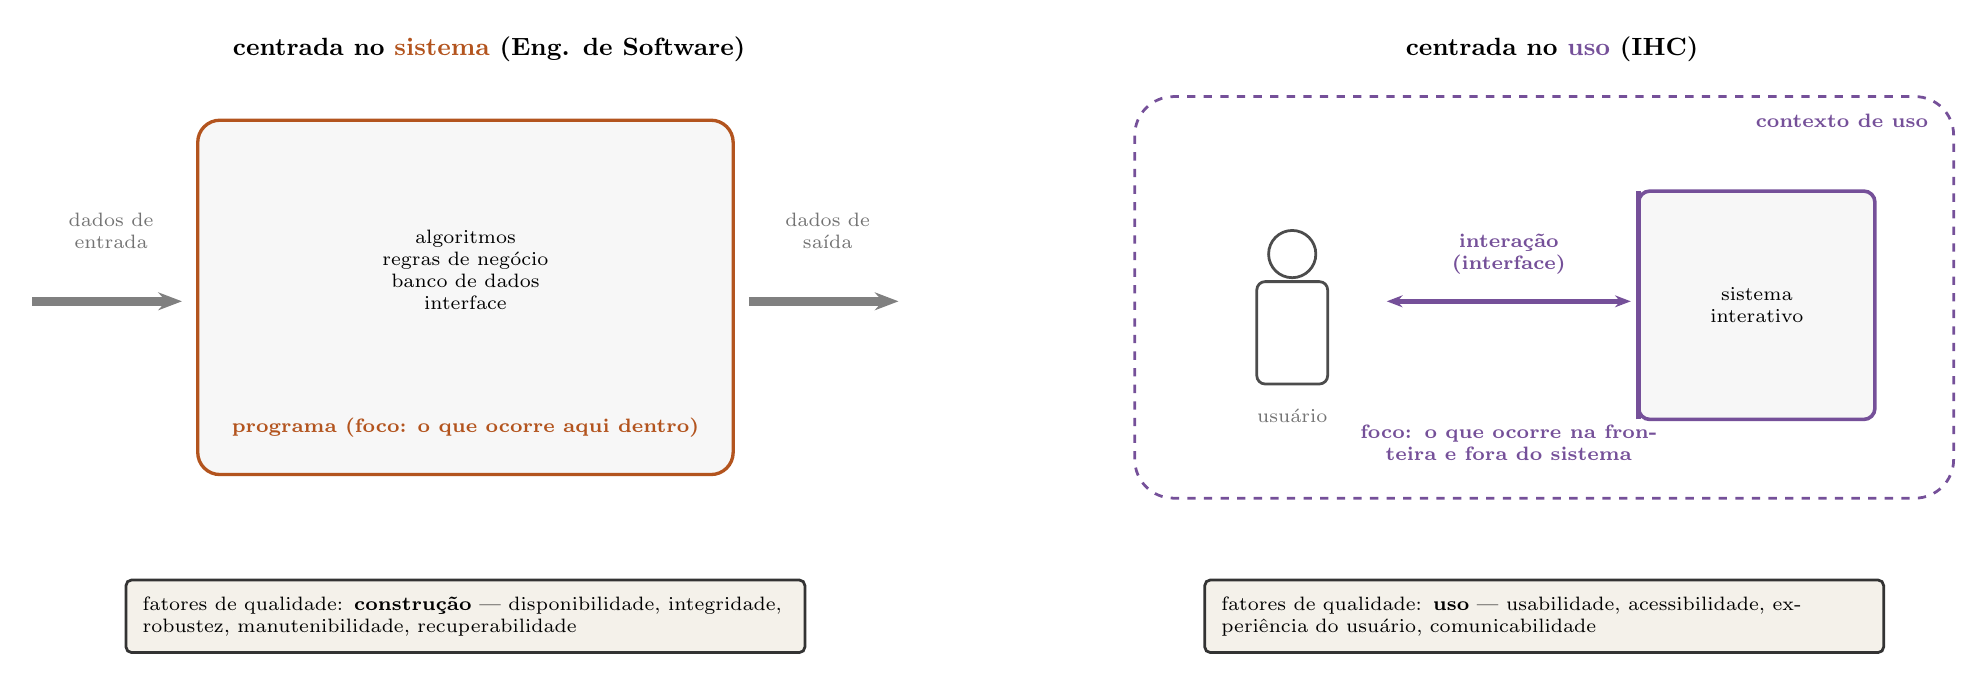
\begin{tikzpicture}[x=1cm,y=1cm]

  % Painel A: centrada no sistema (ES)
  \node[font=\bfseries\small] at (4.5,6.2) {centrada no \textcolor{dorange}{sistema} (Eng. de Software)};
  \draw[-{Stealth[length=3mm]}, black!50, line width=3.4pt] (-1.3,3) -- (0.6,3);
  \node[dlbl, font=\scriptsize, align=center] at (-0.3,3.9) {dados de\\entrada};
  \draw[dbody, rounded corners=8pt, line width=1.2pt, draw=dorange] (0.8,0.8) rectangle (7.6,5.3);
  \node[font=\scriptsize, align=center, text width=5.6cm] at (4.2,3.4) {algoritmos\\regras de negócio\\banco de dados\\interface};
  \node[dorange, font=\scriptsize\bfseries] at (4.2,1.4) {programa (foco: o que ocorre aqui dentro)};
  \draw[-{Stealth[length=3mm]}, black!50, line width=3.4pt] (7.8,3) -- (9.7,3);
  \node[dlbl, font=\scriptsize, align=center] at (8.8,3.9) {dados de\\saída};

  \node[dbox, text width=8.2cm, font=\scriptsize, align=left] at (4.2,-1.0) {fatores de qualidade: \textbf{construção} --- disponibilidade, integridade, robustez, manutenibilidade, recuperabilidade};

  % Painel B: centrada no uso (IHC)
  \begin{scope}[shift={(13.5,0)}]
    \node[font=\bfseries\small] at (4.5,6.2) {centrada no \textcolor{dblue}{uso} (IHC)};
    \draw[dblue, dashed, line width=1pt, rounded corners=14pt] (-0.8,0.5) rectangle (9.6,5.6);
    \node[dblue, font=\scriptsize\bfseries, anchor=north east] at (9.4,5.5) {contexto de uso};

    \begin{scope}[shift={(1.2,2.3)}]
      \draw[black!70, line width=1pt, fill=white] (0,1.3) circle (0.3);
      \draw[black!70, line width=1pt, fill=white, rounded corners=3pt] (-0.45,-0.35) rectangle (0.45,0.95);
      \node[dlbl, font=\scriptsize] at (0,-0.75) {usuário};
    \end{scope}
    \draw[dbody, rounded corners=4pt, draw=dblue, line width=1.3pt] (5.6,1.5) rectangle (8.6,4.4);
    \node[font=\scriptsize, align=center, text width=2.6cm] at (7.1,2.95) {sistema\\interativo};
    \draw[dbody, draw=dblue, line width=1.8pt] (5.6,1.5) -- (5.6,4.4);
    \draw[<->, dblue, line width=1.6pt] (2.4,3.0) -- (5.5,3.0);
    \node[dblue, font=\scriptsize\bfseries, align=center] at (3.95,3.6) {interação\\(interface)};
    \node[dblue, font=\scriptsize\bfseries, align=center, text width=5cm] at (3.95,1.2) {foco: o que ocorre na fronteira e fora do sistema};

    \node[dbox, text width=8.2cm, font=\scriptsize, align=left] at (4.4,-1.0) {fatores de qualidade: \textbf{uso} --- usabilidade, acessibilidade, experiência do usuário, comunicabilidade};
  \end{scope}

\end{tikzpicture}
\end{document}
